\documentclass[final,pdftex]{../../template/epsilonj}

\RequirePackage{graphicx}

\usepackage{listings}
\RequirePackage[colorlinks,citecolor=blue,urlcolor=blue]{hyperref}

\addbibresource{../../template/epsilon.bib}

\newcommand{\mydiv}{\nonscript \mskip -\medmuskip \mkern 5mu \mathbin {\rm div}\penalty 900\mkern 5mu\nonscript \mskip -\medmuskip}

\begin{document}
\setcounter{page}{37}
	
	% \microtypesetup{protrusion=false, expansion=false}
	\begin{frontmatter}
		\title{QR-код, или немного о дополненной реальности}
		\runtitle{QR-код, или немного о дополненной реальности}
		
		\begin{aug}
			\author{\imya{Настя} \fam{Игнатьева}}%
			
			\runauthor{Настя Игнатьева}
			
			\address{НИУ ВШЭ, Москва.}
		\end{aug}
		
		\begin{abstract}
			Статья знакомит читателей с одной из наиболее известных разновидностей дополненной реальности --- QR-кодам. Помимо основных технических характеристик Вы сможете узнать, как устроен QR-код, понять алгоритмы, которые используются при шифровании информации, а также, как декодировать QR-код вручную. 
		\end{abstract}
		
		\begin{keyword}
			\kwd{дополненная реальность}
			\kwd{QR-код}
			\kwd{распознавание образов}
		\end{keyword}
		
	\end{frontmatter}
	
	
	\section{Раздел 1}


Что позволяет порядочному исследователю творить? Совесть?  Возможно, но здесь не об~этом, здесь всё серьёзно. Это \textit{данные}. Сегодня они нужны всем, ведь любой эконометрический анализ, как и~множество исследований, без этого ключевого элемента становится невозможным или остаётся узником чистой и~неприменимой теории. Вот так в~поисках релевантных временных рядов, всевозможных панелей и~просто данных мы скитаемся по интернету: \href{http://www.fira.ru}{fira.ru}, незаменимый \href{http://www.gks.ru}{gks.ru}, различные базы OECD, RUSLANA, СПАРК\ldotst{} Впрочем, это не новость, собственно, и~заметка не совсем об~этом. Всё дело в~том, что мало кто замечает: данные повсюду, нужно только заглянуть несколько глубже, заглянуть в~дополненную реальность. 

После того как необходимая, хоть и~минимальная, отсылка к~эконометрике, ввиду тематики журнала, была соблюдена, самое время поговорить об~этой самой дополненной реальности, где окружающий нас мир соприкасается с~миром виртуальным.

Почему именно дополненная реальность? Просто мне всегда казалось, что это слишком сложно, чтобы быть правдой. Возможно, для девушек это вполне нормально, когда компьютер почти как магия.

\begin{figure}[htbp]
\centering 	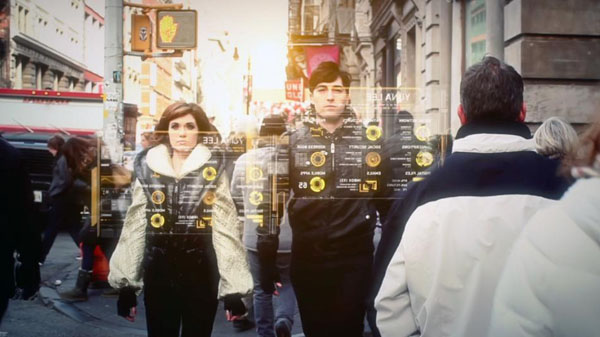
\includegraphics[width=90mm]{1.jpg}
\caption{Дополненная реальность} 
\end{figure}

Всё началось с~машинного зрения. Для человека зрение настолько естественно, что большинство просто не задумывается, что кого-то, в~данном случае что-то, нужно этому учить. Хотя многие современные компьютеры выглядят совсем не глупее людей, научить их видеть "--- чрезвычайно непростая задача. Они должны не только уметь различать цвета, идентифицировать предметы, определять их границы и~классифицировать, но и~учитывать контекст, внутриклассовую изменчивость, масштаб, освещение, возможную деформацию при движении, изменении ракурса и~положения, отличать, к~примеру, отбрасываемую тень от самого предмета.
%\begin{figure}[htbp]
%\centering 
%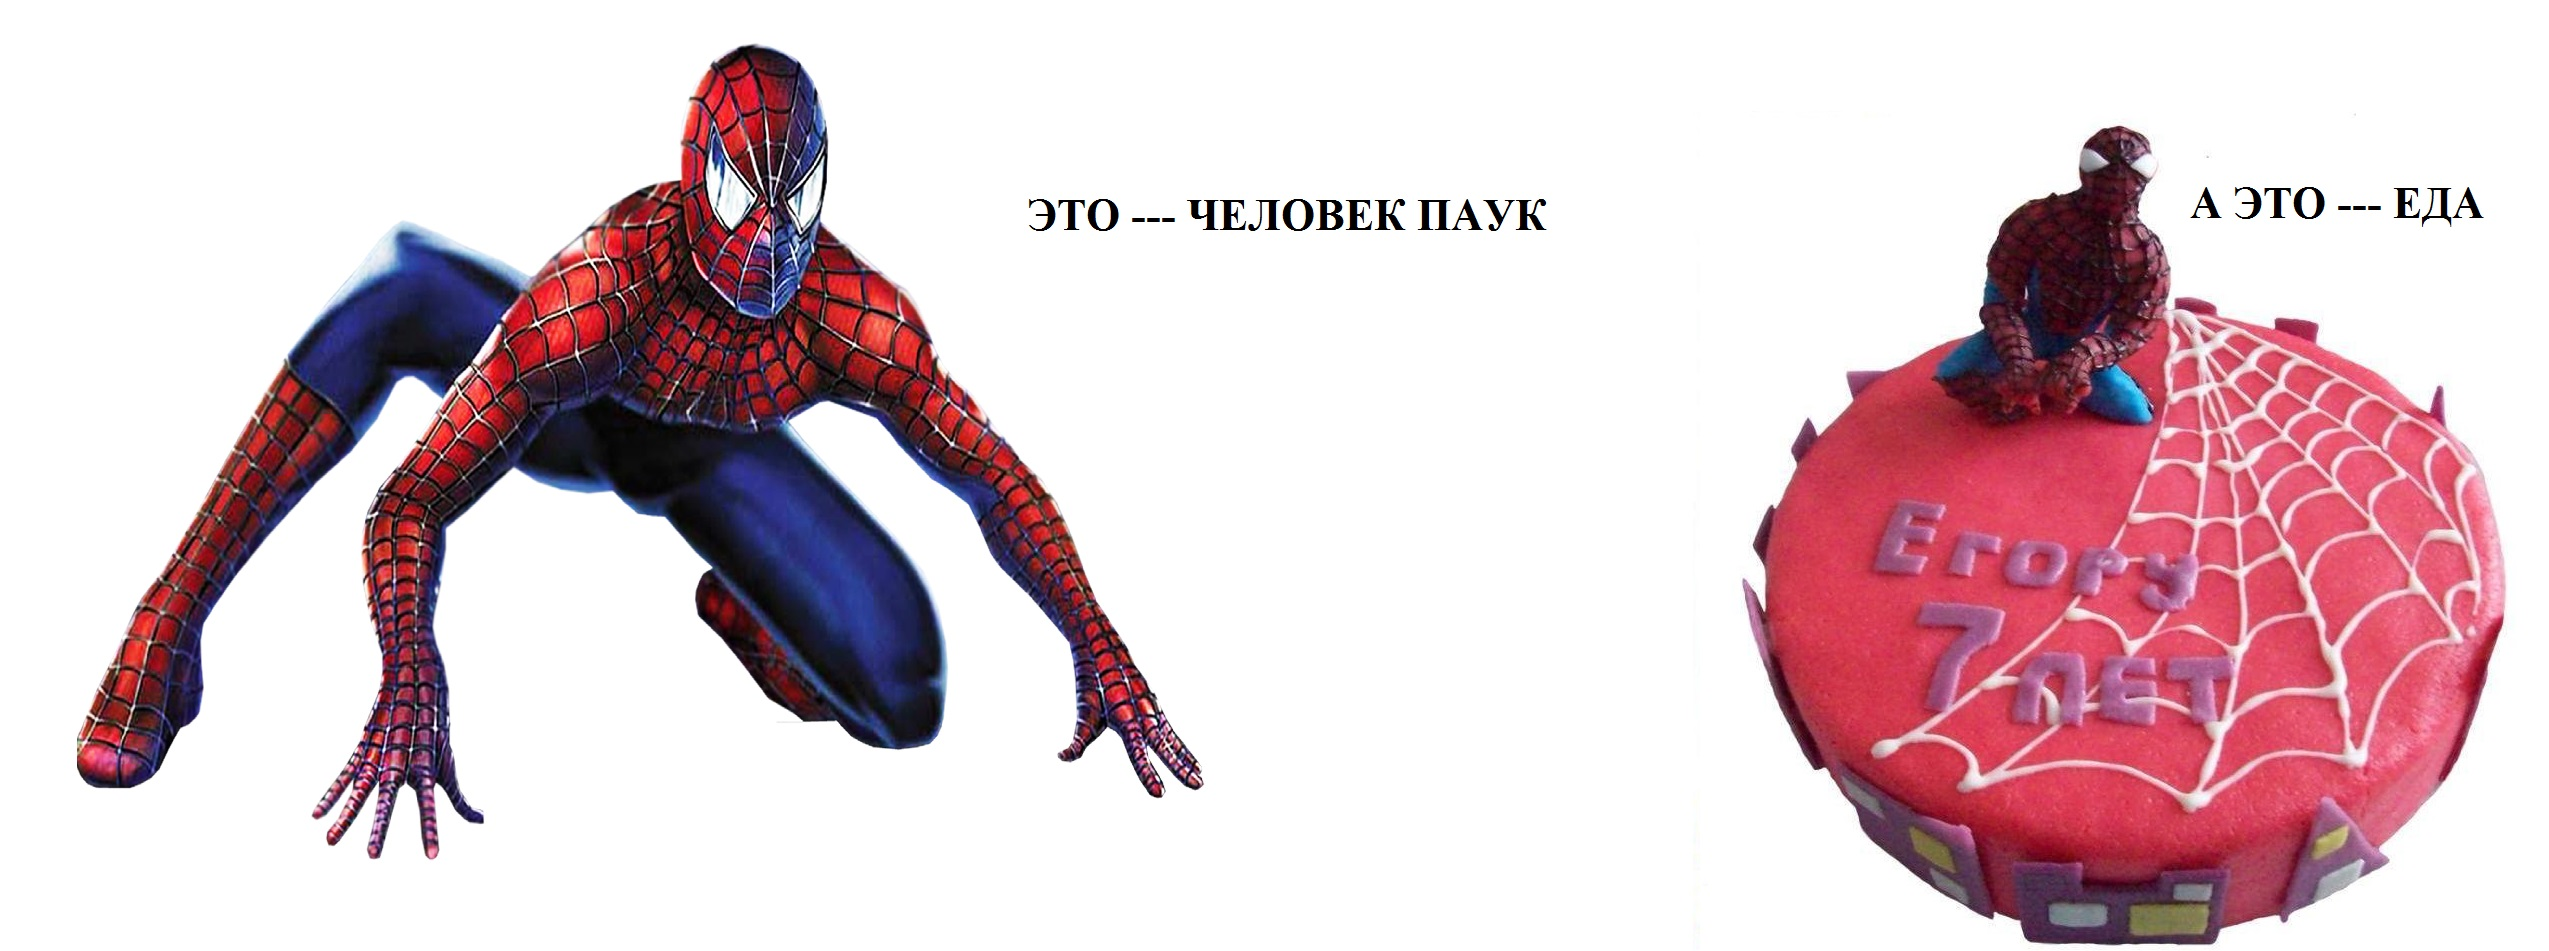
\includegraphics[width=50mm]{tt.jpg}\quad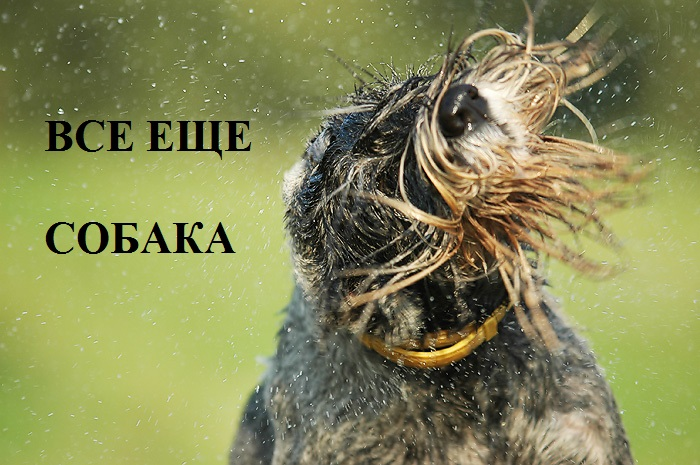
\includegraphics[width=50mm]{dd.jpg}
%\caption{Заголовок 2}
%\end{figure}

Однако мир не без умных людей, и~современные алгоритмы так или иначе позволяют решать эти проблемы. Сфера применения компьютерного зрения весьма обширна: системы моделирования объектов и~окружающей среды, медицинских изображений (рентген, томография), системы видеонаблюдения и~организации информации, а~также системы дополненной реальности и~проч. С~дополненной реальностью, несмотря на всю загадочность названия, сталкивался каждый, кто хоть раз смотрел различные спортивные мероприятия, будь то теннис, когда в~случае спорных моментов моделируется траектория полёта мяча, или футбол, где при определении офсайда возникает линия, параллельная лицевой, которая позволяет определить ближайшего к~воротам игрока.

Одна из разновидностей дополненной реальности "--- это всем известные QR-коды и~штрихкоды. Несложно догадаться, гд\'{е} именно черпал вдохновение создатель штрихкодов: да, вы правы, в~азбуке Морзе. Однако линейные штрихкоды вмещают слишком мало информации "--- по этой причине в~1994~году в~Японии и~были изобретены двухмерные, или матричные коды, самым популярным из которых и~стал QR-код, что означает «быстрый отклик» (\ENGs{Quick Response}). Если у~обычных штрихкодов объём памяти не превышал 100~байт, то у~матричных кодов данный показатель значительно выше "--- до 2048~байт (\cite{WikiDataMatrixRu}); более того, информация может быть считана даже при 30\%-м повреждении метки! 

Сегодня QR-коды можно встретить где угодно, даже на~кладбищах, где данные коды используются для хранения информации об~усопшем. Такое нестандартное решение относительно применения QR-кодов было найдено в~Японии и~Австралии, впрочем, вернемся к~основным техническим характеристикам.  Самый маленький QR-код имеет размер $21\times21$ пиксель, в~то время как самый большой (версия~40) "--- $177\times177$ пикселей. Что касается кодировки QR"=кодов, то существует 4~основных типа: цифровая (до~7089~цифр), алфавитно"=цифровая (до~4296~символов), байтовая (до~2953~байт), кандзи (до~1817~иероглифов) (\cite{WikiQRCodeRu}).

Каждому не раз приходилось сталкиваться с~QR-кодами в~жизни, некоторые даже использовали смартфоны, чтобы считать код. Но вряд ли кому-то приходило в~голову делать это вручную. А~так как в~жизни бывают разные ситуации, почему бы не восполнить данный пробел?

Для начала разберёмся, как устроен QR-код. Изначально данные, которые нужно закодировать, разбиваются на блоки в~зависимости от режима кодирования; далее прибавляется заголовок, указывающий режим и~количество блоков. Безусловно, существуют режимы с~более сложной структурой кодирования, однако из них весьма проблематично извлекать информацию вручную, поэтому остановимся на более простых случаях. После того как записаны все информационные данные, к~ним добавляются корректирующие ошибки коды Рида"--~Соломона (RS), которые позволяют исправлять недочёты при чтении. Именно эти коды и~занимают большую часть QR"=матрицы. Перед записью в~картинку данные с~RS"=кодами перемешиваются, для чего используются специальные маски. Среди имеющихся восьми алгоритмов, которые представлены на рис.~\ref{fig:8algs}, выбирается наилучший, который определяется за счёт системы штрафов. После этой процедуры перемешанные данные записываются на шаблонную картинку, к~которой добавляется техническая информация для декодирующих устройств (\cite{HabrQRcode}).

\begin{figure}[hbt]
			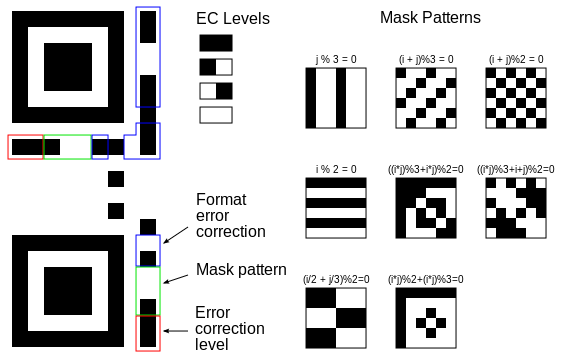
\includegraphics[width=90mm]{qr2.png}
			\caption{Восемь алгоритмов масок}\label{fig:8algs}
\end{figure}

Возможно, многие замечали, что QR-код можно разбить на несколько областей, у~каждой из которых индивидуальные функции (показано на рис.~\ref{fig:oblasti}). Так вот, три квадрата в~углах изображения и~меньшие синхронизирующие квадратики по всему коду и~суть техническая информация для декодирующих устройств, которая позволяет нормализовать размер изображения и~его ориентацию, а~также угол, под которым сенсор расположен к~поверхности изображения. Таким образом, как вы можете догадаться, эта область абсолютно неинтересна для нас, так как не содержат никакой информации о~скрывающемся за кодом послании. Что касается полезной части кода, то её можно разделить на две области: область, отвечающая за системную информацию, и~непосредственно данные. Также в~матрице содержится информация о~версии кода, от которой зависит ёмкость последнего. Так, при повышении версии добавляются специальные блоки; при высоких версиях кода не рекомендуется считывать его вручную.

\begin{figure}[hbt]
			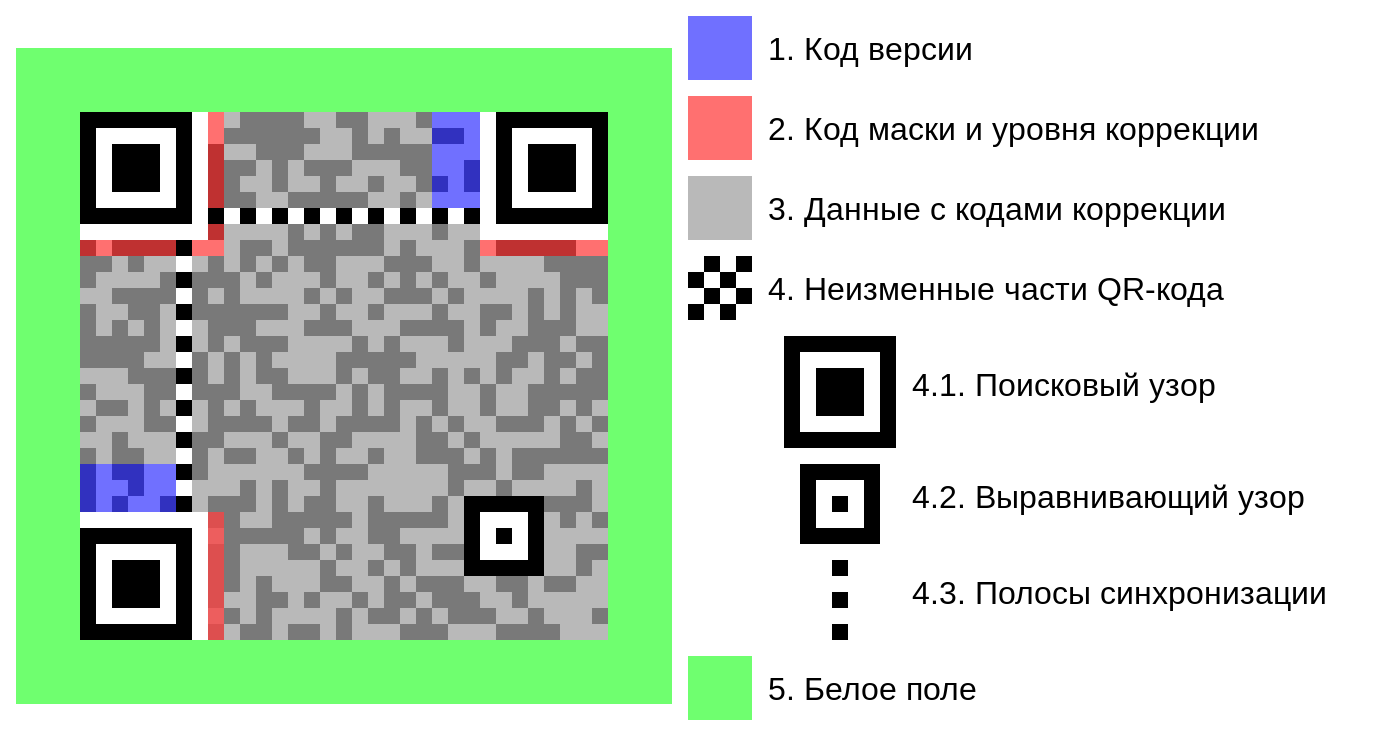
\includegraphics[width=90mm]{qr1.png} 
			\caption{Области QR-кода}\label{fig:oblasti}
\end{figure}

Системная информация представляет собой 15~бит данных, из которых только 5~бит для нас значимы: 2~бита отвечают за уровень коррекции ошибок, а~оставшиеся~3 "--- за применяемую к~данным маску. Ещё 10~бит данных "--- это BCH"=код,  так называемый код Боуза-Чоудхури-Хоквингема, который относится к широкому классу циклических кодов и позволяет исправлять ошибки в~системных данных.  Упомянутые ранее RS"=коды, коды Рида"--~Соломона, также относятся к~классу BCH. Помимо всего прочего, для дополнительной защиты системной информации используется статическая маска, применяемая к~любой системной информации. Она имеет запись 101010000010010. Так как нам интересны только первые 5 бит, то маску можно сократить, и~её уже не так сложно запомнить: 10101. Как видно из рисунка, системная информация, отмеченная красным цветом, дублируется, что позволяет значительно понизить вероятность возникновения ошибок.


Таким образом, \textbf{первый шаг "--- чтение первых 5~бит системной информации} (рис.~\ref{fig:fivebits}).
\begin{figure}[htbp]
	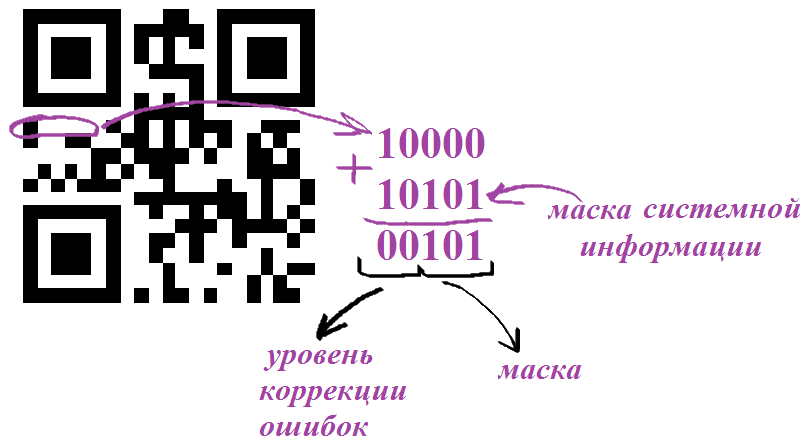
\includegraphics[width=70mm]{1.png}
	\caption{Чтение первых 5~бит информации}\label{fig:fivebits}
\end{figure}

Для лучшего понимания воспользуемся кодом, сгенерированным на \href{http://qrcoder.ru}{\ENGs{qrcoder.ru}}. Получили, что для нашего кода уровень коррекции ошибок "--- 00 "--- уровень М, позволяющий скорректировать до 15\,\% ошибок, маска "--- 101, соответствующая 8-й схеме на рисунке~\ref{fig:8algs}. Все возможные варианты масок и~уровней коррекции представлены в~таблице~\ref{tab:mlt}.

\textbf{Шаг второй "--- определение режима кодировки.}
\begin{figure}[hbt]
	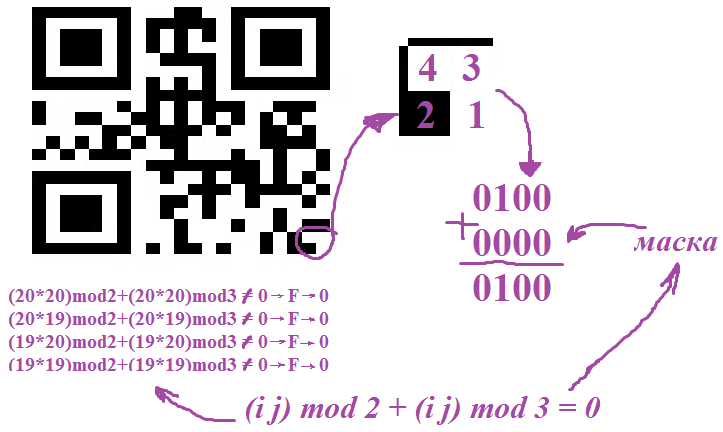
\includegraphics[width=90mm]{21.png}
	\caption{Определение режима кодировки}
\end{figure}

Чтобы понять, с~какими данными предстоит иметь дело, необходимо изначально прочитать 4"=битный заголовок, который содержит в~себе информацию о~режиме. Заголовок находится в~правом нижнем углу матрицы, причём читать его надо змейкой, начиная справа. После извлечения четырёх бит, описывающих режим, необходимо применить к~ним маску. Маска определяется выражением, приведённым в~таблице "--- в~нашем случае
\[
(i j) \bmod 2 + (i j) \bmod 3 = 0.
\]
Если данное выражение сводится к~\textsf{TRUE} для бита с~координатами $(i;j)$, то бит инвертируется, иначе всё остаётся без изменений. Начало координат "--- в~левом верхнем углу, $(0;0)$; в~матрице $21\times21$ бит, т.\,е. квадрат; таким образом, бит, находящийся в~правом нижнем углу, имеет координаты $(20;20)$. Получили 0100, что соответствует 8"=битному режиму.

\textbf{Шаг третий "--- чтение данных.}
\begin{figure}[hbt]
	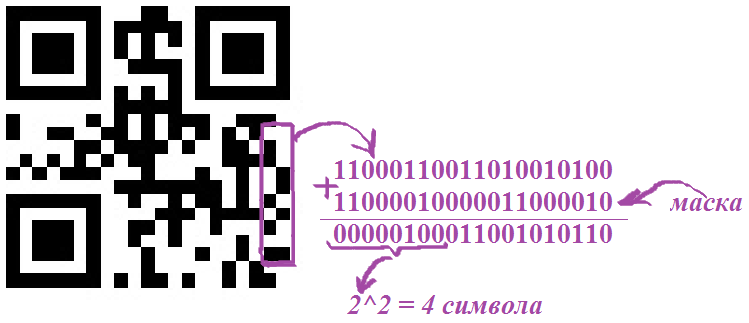
\includegraphics[width=80mm]{31.png}
	\caption{Чтение данных}
\end{figure}

Необходимость определения режима кодирования обуславливается тем, что от него зависит длина блоков данных, которая также варьируется для различных версий кода. Для версий кода 1--9 в~числовом режиме используются 10- или 4"=битные блоки (последние "--- если в~10"=битном объёме нет необходимости); в~буквенно"=числовом режиме "--- 9"=битные блоки; в~8"=битном (байтном) режиме "--- 8-битные блоки. Первый блок после указателя режима "--- это количество символов. Таким образом, для определения количества символов расшифровываем следующие 8~бит кода (змейкой, начиная справа) и~применяем маску. Видно, что в~коде зашифровано 4~символа, поэтому необходимо перейти к~чтению следующего столбца для извлечения всех четырёх блоков информации.

\begin{figure}[htbp]
	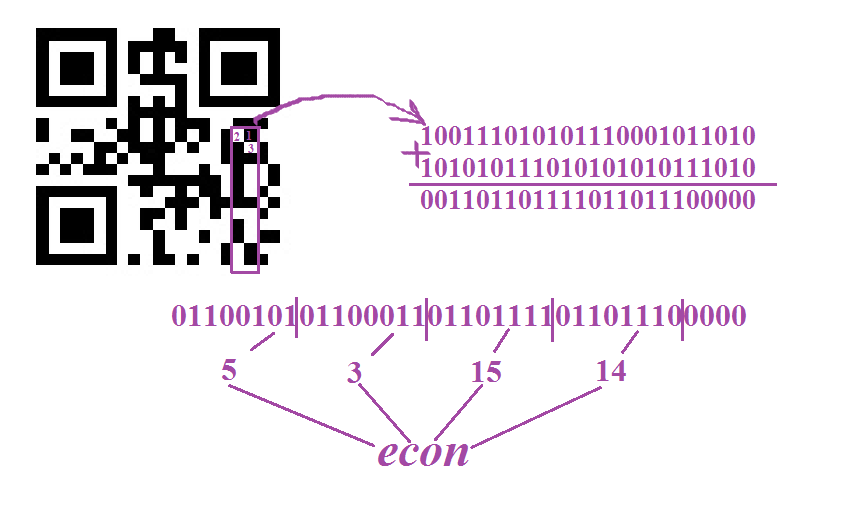
\includegraphics[width=80mm]{41.png}
	\caption{Расшифровка ASCII-кода}
\end{figure}

Снова считываем данные по такому же алгоритму. Главное отличие: биты надо отсчитывать змейкой, но с~правого верхнего угла. Далее полученный набор из нулей и~единиц делим на 4~блока по 8~бит в~каждом. Текст в~8-битном режиме многие онлайн"=генераторы QR"=кодов кодируют, используя ASCII. Таким образом, первые 4~элемента блока указывают на регистр, 0110 соответствует нижнему регистру букв, 0100 "--- верхнему, вторые 4 элемента "--- это число, равное номеру буквы в~алфавите. Как можно заметить, все наши буквы строчные. Получаем числа 5, 3, 15 и~14 и~находим нужные нам буквы. Так, в~коде была зашифрована часть слова, а~именно \textbf{econ}, а~какого именно слова "--- \ENGs{economics}, или \ENGs{econometrics}, или что-то ещё "--- пусть каждый решает для себя сам!


\begin{table}[hbtp]
\centering
\begin{tabular}{||c|l||}
\hline 
\multicolumn{2}{|c|}{\bf Возможные маски}\\ 
\hline
{\bf 000} & $(i + j) \bmod 2 = 0$ \\
{\bf 001} & $i \bmod 2 = 0$ \\
{\bf 010}	& $j \bmod 3 = 0$ \\
{\bf 011}	& $4(i + j) \bmod 3 = 0$ \\
{\bf 100}	& $((i \mydiv 2) + (j \mydiv 3)) \bmod 2 = 0$ \\
{\bf 101}	& $(i j) \bmod 2 + (i j) \bmod 3 = 0$ \\
{\bf 110}	& $((i j) \bmod 2 + (i j) \bmod 3) \bmod 2 = 0$ \\
{\bf 111}	& $((i+j) \bmod 2 + (i j) \bmod 3) \bmod 2 = 0$ \\
\hline 
\multicolumn{2}{|c|}{\bf Возможные уровни коррекции ошибок}\\  
\hline
{\bf  01} & L\\
{\bf  00} & M\\
{\bf  11} & Q\\
{\bf  10} & H\\
\hline
\multicolumn{2}{|c|}{\bf Возможные режимы}\\  
\hline
{\bf  0111} & ECI\\
{\bf  0001} & Числовые\\
{\bf  0010} & Буквенно-числовые\\
{\bf  0100} & 8-битный (байтный)\\
{\bf  1000} & Kanji\\
{\bf  0011} & Структурированное дополнение\\
{\bf  0101} & FNC1 (1-я позиция)\\
{\bf  1001} & FNC1 (2-я позиция)\\
\hline
\end{tabular}
\caption{Варианты масок и уровней коррекции} \label{tab:mlt}
\end{table}

\printbibliography

\begin{center}
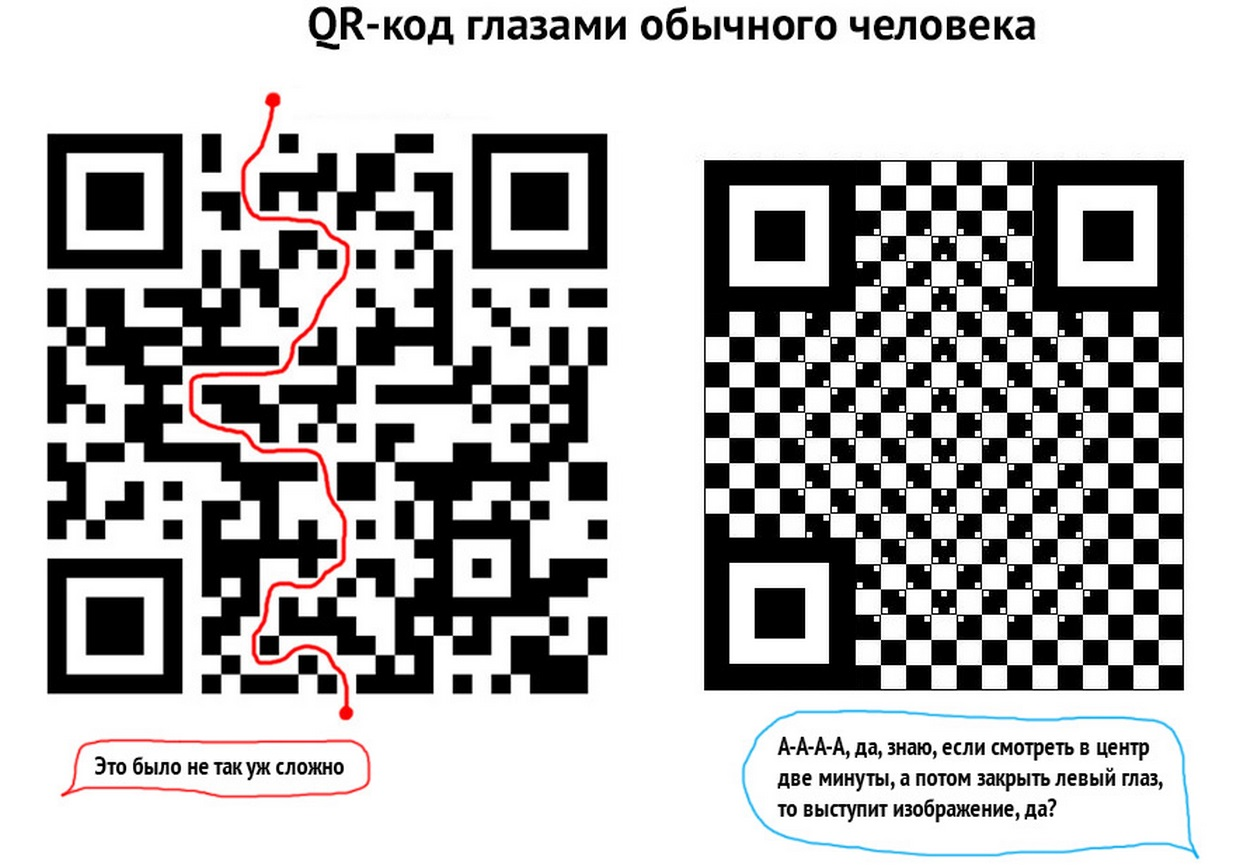
\includegraphics[width=87mm]{qr.jpg} 
\end{center}



\end{document}